% ****** Start of file apssamp.tex ******
%
%   This file is part of the APS files in the REVTeX 4.1 distribution.
%   Version 4.1r of REVTeX, August 2010
%
%   Copyright (c) 2009, 2010 The American Physical Society.
%
%   See the REVTeX 4 README file for restrictions and more information.
%
% TeX'ing this file requires that you have AMS-LaTeX 2.0 installed
% as well as the rest of the prerequisites for REVTeX 4.1
%
% See the REVTeX 4 README file
% It also requires running BibTeX. The commands are as follows:
%
%  1)  latex apssamp.tex
%  2)  bibtex apssamp
%  3)  latex apssamp.tex
%  4)  latex apssamp.tex
%
\documentclass[%
 reprint,
%superscriptaddress,
%groupedaddress,
%unsortedaddress,
%runinaddress,
%frontmatterverbose, 
%preprint,
%showpacs,preprintnumbers,
%nofootinbib,
%nobibnotes,
%bibnotes,
 amsmath,amssymb,
 aps,
%pra,
%prb,
%rmp,
%prstab,
%prstper,
%floatfix,
]{revtex4-1}

\usepackage{graphicx}% Include figure files
\usepackage{dcolumn}% Align table columns on decimal point
\usepackage{bm}% bold math
%\usepackage{hyperref}% add hypertext capabilities
%\usepackage[mathlines]{lineno}% Enable numbering of text and display math
%\linenumbers\relax % Commence numbering lines

%\usepackage[showframe,%Uncomment any one of the following lines to test 
%%scale=0.7, marginratio={1:1, 2:3}, ignoreall,% default settings
%%text={7in,10in},centering,
%%margin=1.5in,
%%total={6.5in,8.75in}, top=1.2in, left=0.9in, includefoot,
%%height=10in,a5paper,hmargin={3cm,0.8in},
%]{geometry}

\begin{document}

\preprint{APS/123-QED}

\title{Introduction to Python}
\author         {U24568 - Computational Physics}
%\email          {fac@mit.edu}
%\homepage       {http://web.mit.edu/fac/www}
\affiliation    {Dr. Karen Masters \\ University of Portsmouth}
\date{\today}


\date{\today}% It is always \today, today,
             %  but any date may be explicitly specified

\begin{abstract}
Summary of lecture notes, a record of instructions for launching python applications, and instructions for the first set of python exercises to work through. 
\end{abstract}

%\pacs{Valid PACS appear here}% PACS, the Physics and Astronomy
                             % Classification Scheme.
%\keywords{Suggested keywords}%Use showkeys class option if keyword
                              %display desired
\maketitle

%\tableofcontents

%%%%%%%%%%%%%%%%%%%%%%%%%%%%%%%%%%%%%%%%%%%%%%%%%%%%%%%%%%%%%%%%%%%%%%%%%%%%%
\section{\label{sec:intro} Introduction to Python}
In this section we gain familiarity with python (specifically python 3), including different methods to run python by working on Physics problems. Remember you have not enrolled on a programming unit -- rather this is ``Computational {\bf Physics}'',  so our emphasis here will be on using computers to solve physical problems. However a good basis in programming will provide both excellent transferable skills, and give you the skills to ensure you physics computing will go smoother (and faster) in the future. We chose to teach in python rather than the Matlab you learned in ``Introduction to Computational Physics'' because: 
\begin{enumerate}
\item it gives you another language to list on you CV
\item it will give you confidence that you can pick up any language you need
\item it is a sought after language by the employers of physicists
\item it's free and open source (you don't need a license like for Matlab). 
\end{enumerate}
%We will also have a short period of Maple to give you an alternative method to do computer algebra which is commonly employed by theoretical physicists, and during discussions on accuracy and speed of particularly high performance computing you will also have some exposure to the Fortran language. 

%\begin{figure}
%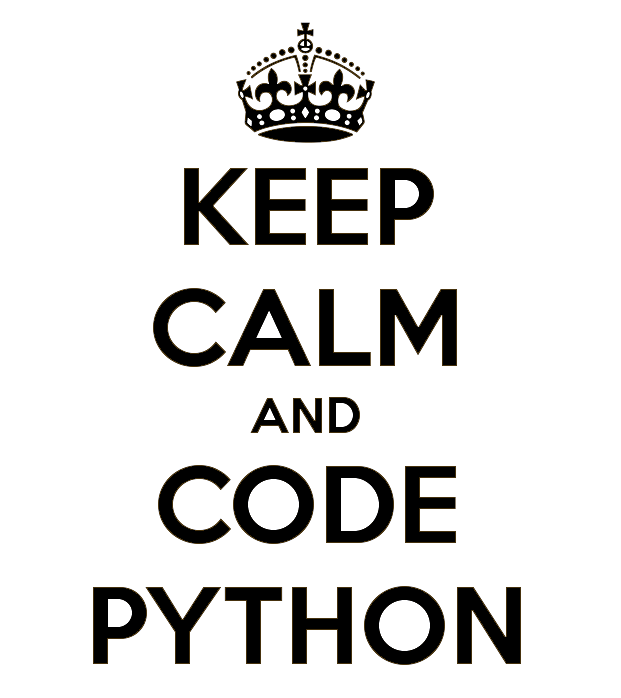
\includegraphics[width=0.40\textwidth]{KeepCalmCodePython.png}%
 %\caption{\label{}}
%\end{figure}

\section{Installing Python \label{sec:install}} 

By far the simplest method to run python for scientific use is via the Anaconda distribution, which uses all the commonly known scientific packages such as Matplotlib, Scipy, Numpy, and takes care of all the relevent dependencies for you. It also comes with different ways to interact with python (see below). 

\subsection{University Networked Computer: Windows}
The Anaconda is ready installed. To access this: 
\begin{itemize}
\item Launch  ``Aps Anywhere"
\item Search for ``Anaconda" (worth ``favouriting" it by clicking on the star)
\item Launch ``Anaconda" (this takes a while first time, and has a bunch of warnings, just keep and eye and click OK; it'll be quicker in future)
\item Launch Jupyter Notebook
\end{itemize}

\subsection{Your own computer/laptop}

You may wish to download Anaconda. It is free and available for Windows, OSX and Linux installation. Make sure you make a python3 environment. 

\subsection{Via SciServer Computer}
This allows you to run python3 in Jupyter notebooks on any computer/device linked to the internet. It's also linked to some large astronomical databases. 
\begin{itemize}
\item Navigate to {\tt http://www.sciserver.org/} and make a (free) account
\item Select ``Compute"
\item Start a ``New Container"
\item Start a python3 Notebook (from the dropdown ``New" menu at upper right).
\end{itemize}

\section{Running Python}

There are many different methods to run python programmes. In Anaconda the three ways you can work with python are directly from the command line (teminal window); using the Interactive Data Environment ``Spyder" (which is supposed to look at lot like Matlab); and using Jupyter Notebooks. The code you write will be identical, just the way you work on it, and run it may differ. 

\subsection{Juptyer Notebooks}

Jupyter Notebooks are web based application which provide a way to create and share documents, which contain live, updateable code. Juptyer can be used with multiple languages, but we'll focus on using it with python. Jupyter is included in the Anaconda distribution, and available online in SciServer. This is an excellent way to write code in a class as it allows you to integrate your notes with the code. 

To launch Jupyter Notebook from a Portsmouth Networked Windows Machine (after you have launched Anaconda): 
\begin{itemize}
\item Start Anaconda (see above), and in Anaconda Navigator Launch Jupyter Notebook. This should open a browser window from the Jupyter Server. 
\item Tip: Make a folder on your account called ``Computational Physics"
\item Navigate to ``Computational Physics" in the Jupyter Browser
\item Start a New Python 3 Notebook (from the menu at upper right).
\item To end select ``Close and halt" from the file menu
\end{itemize}

Let's try this: 
\begin{enumerate}
\item Start up a Jupyter Notebook (see above, or use SciServer).
\item In the first box write a title (e.g. ``Python notes"), and some notes on what we're doing (change this to a ``Markdown" box).
\item In the second box write {\tt print("Hello World")} and run it. 
\item "Save and Checkpoint" (from the File Menu). Do this frequently. 
\item Now work through the beginning of the Python Programming for Physicists tutorial (Chapter 2 of Newman \cite{newman}) from Section 2.2 up to and including Exercise 2.2: ``Calculating the Altitude of a Satellite" writing the code and notes on it in a Juptyer Notebook.
\end{enumerate}


\subsubsection{Github}
 One nice feature of Jupyter Notebooks is how they enable the sharing of code (and outputs) via platforms like ``Github" ({\tt http://github.com}. I encourage you to get an account on ``Github" and start a repository for your Computational Physics work. Later in the term I will be using Github to share my own Notebooks of example code. You can find my ``Computational Physics Unit" repository at {\tt github.com/karenlmasters/ComputationalPhysicsUnit}. 

\subsection{Spyder} 

Spyder is the Scientific PYthon Development EnviRonment. It's one of many Integrated Development Environments for the python language, and it's distributed with the Anaconda python package. I have been told it's quite similar to the Matlab Development Environment, so this may be the most familiar way for you to run python. However as 2nd year physicists I'd like to encourage you to not use a GUI environment like this - my examples will all be in Jupyter Notebooks. 

%\begin{enumerate}
%\item Start up Spyder (type {\tt spyder} in the terminal).
%\item Work through the beginning of the Python Programming for Physicists tutorial (Chapter 2 of Newman \cite{newman}) up to and including Exercise 2.2: "Calculating the Altitude of a Satellite" using Spyder as your IDE (instead of IDLE as suggested in the Chapter). 
%\end{enumerate}


\subsection{Command Line}

For completeness I wish to mention this method of using python, which will be easiest if done under linux (or Mac). Any python code saved in a ``code.py'' file (where ``code'' is just any name you choose) can be run this way. There are linux text editors (e.g. {\tt nano} which can edit these files directly (note that Jupyter Notebook include formatting content which will not work - you need to copy and paste just the coding parts of the Notebook to do this)

To run code at the command line you simply type: 

\begin{verbatim}
> python code.py
\end{verbatim}

(where {\tt code.py} is the file name of your python code). This is most useful for code which takes a long time to run, or which you need to run with different inputs. Most experienced coders I know use this method (although Jupyter Notebooks are becoming more common). 

%Write a simple ``I love Physics" code (ie. a code which runs and prints ``I love Physics" to the terminal) in a text editor to run from the command line. 

Tip: there are more advanced text editors available in Linux which colour code the coding syntax. I often use a version of Emacs to write code for this reason. 



\section{Python for Physics Tutorial}

Now please work through the remainder of Chapter 2 of Newman \citep{newman} using the python interface of your choice. 

Tips: 
\begin{itemize}
\item Save your Notebook with names you remember (e.g. NewmanChapter2) 
\item Give your variables sensible names (so you can remember what they are)
\item Your code will be more efficient (and less bug prone) if you define variables to have the correct types (integer/floating etc). 
\item Mistakes and error messages are normal in programming, and working out what they mean can be tricky (but is not impossible). Google (or your search engine of preference) will be your friend here, as will asking your peers (and your lecturers) for help. 
\end{itemize}

%%%%%%%%%%%%%%%%%%%%%%%%%%%%%%%%%%%%%%%%%%%%%%%%%%%%%%%%%%%%%%%%%%%%%%%%%%%%%
%\section{Physics Examples for your Portfolio}

%Please work through the following exercises writing commented code (as Jupyter Notebooks) to hand in for your portfolio. 
%Please use all three methods we have been practicing to interact with Python (i.e. write one as a Python script in a text editor to run, do one in the Spyder IDE and one as a Jupyter Notebook. You may choose which method to run the fourth, exercise but please explain your choice. There is no correct answer, it's simply a function of programming style and personal preferences). 

%2016
%1. Calculating the Altitude of a Satellite - Exercise 2.2 (Newman \citep{newman}, pg 30) 
%2. Quantum potential step - Exercise 2.5  (Newman \citep{newman},  pg 36) - 
%3. The semi-empirical mass formula - Exercise 2.10  (Newman \citep{newman},  pg 75)
%4. Make a user defined function to calculate binomial coefficients - Exercise 2.11 (Newman \citep{newman},  pg 82) 

%\begin{figure*}
%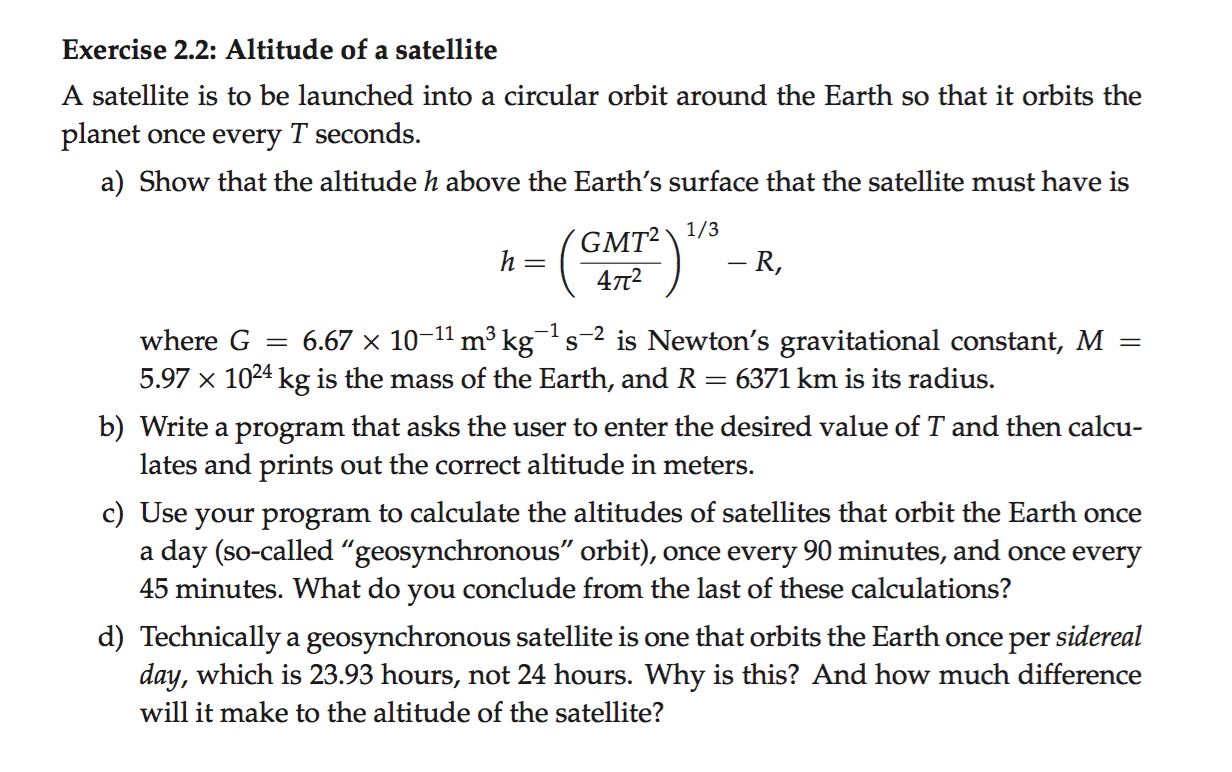
\includegraphics[width=1.0\textwidth]{Exercise2_2.png}%
 %\caption{\label{}}
%\end{figure*}

%\begin{figure*}
%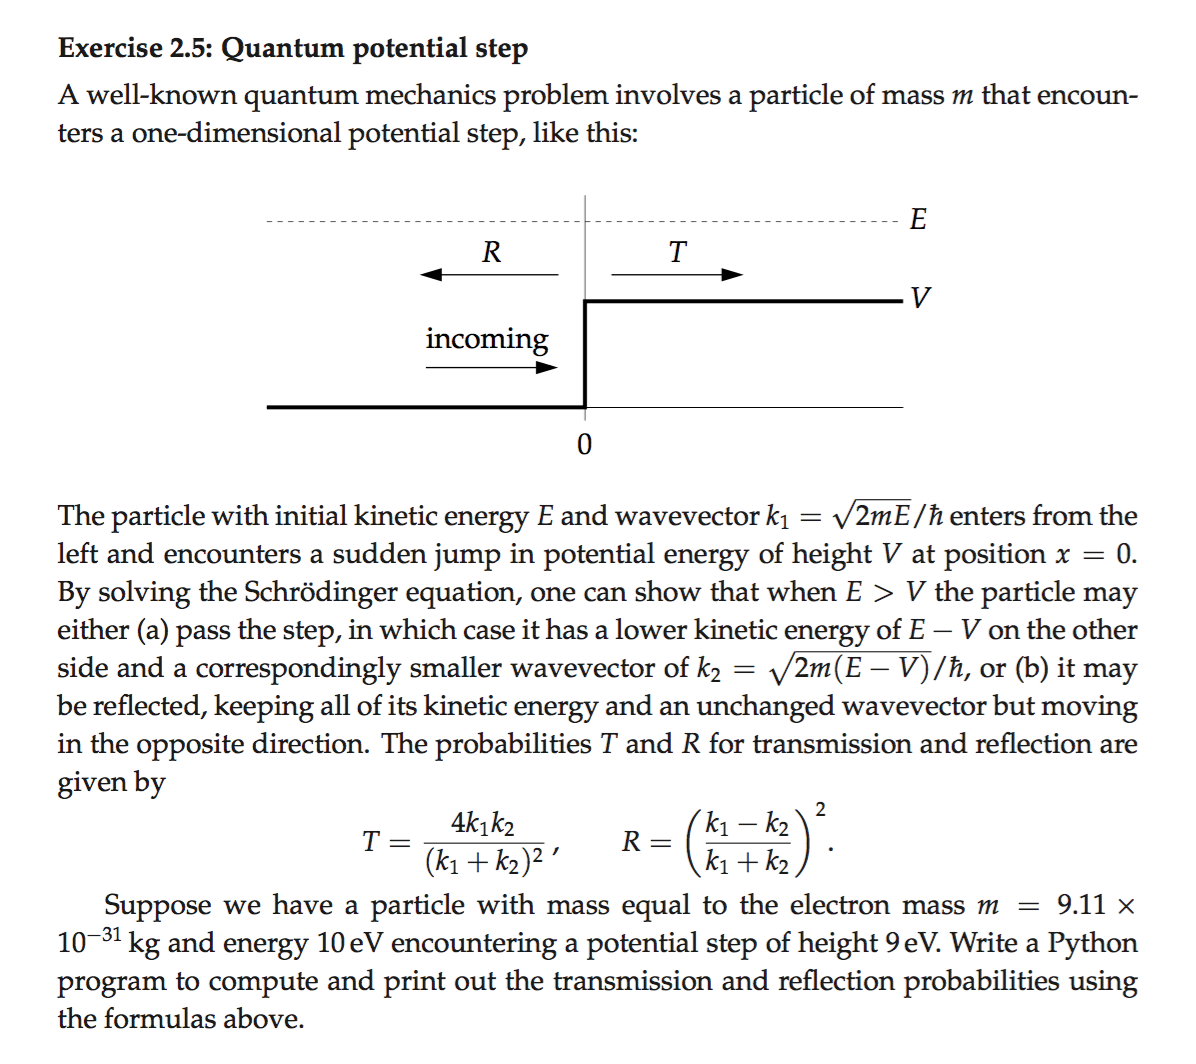
\includegraphics[width=1.00\textwidth]{Exercise2_5.png}%
 %\caption{\label{}}
%\end{figure*}

%\begin{figure*}
%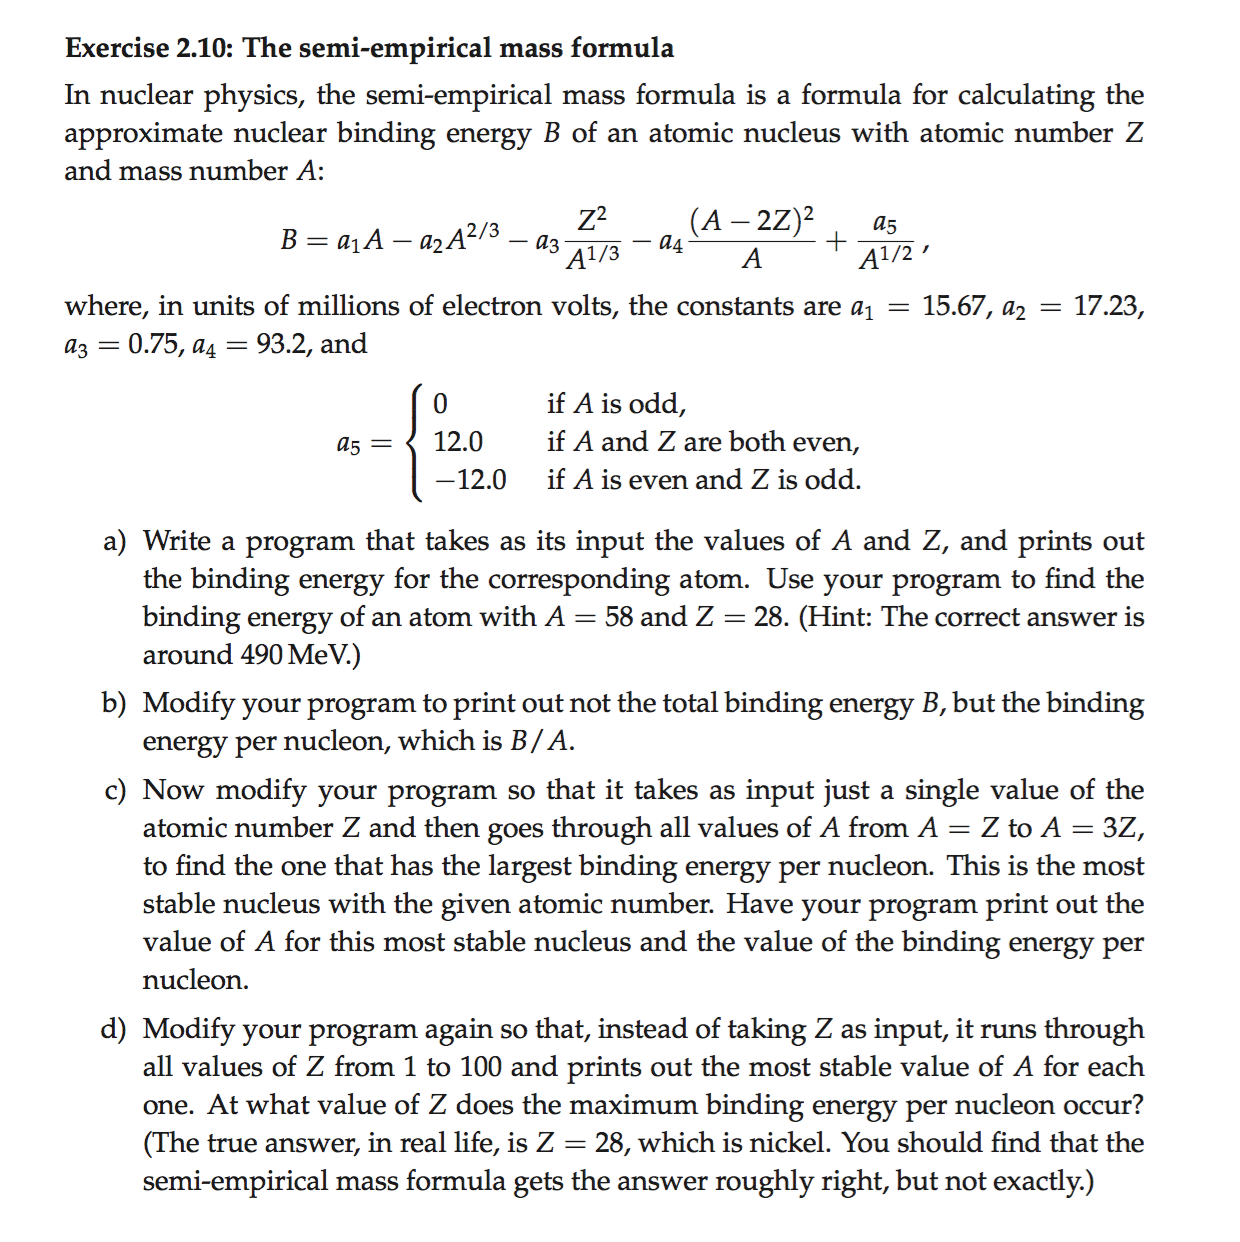
\includegraphics[width=1.0\textwidth]{Exercise2_10.png}%
 %\caption{\label{}}
%\end{figure*}

%\begin{figure*}
%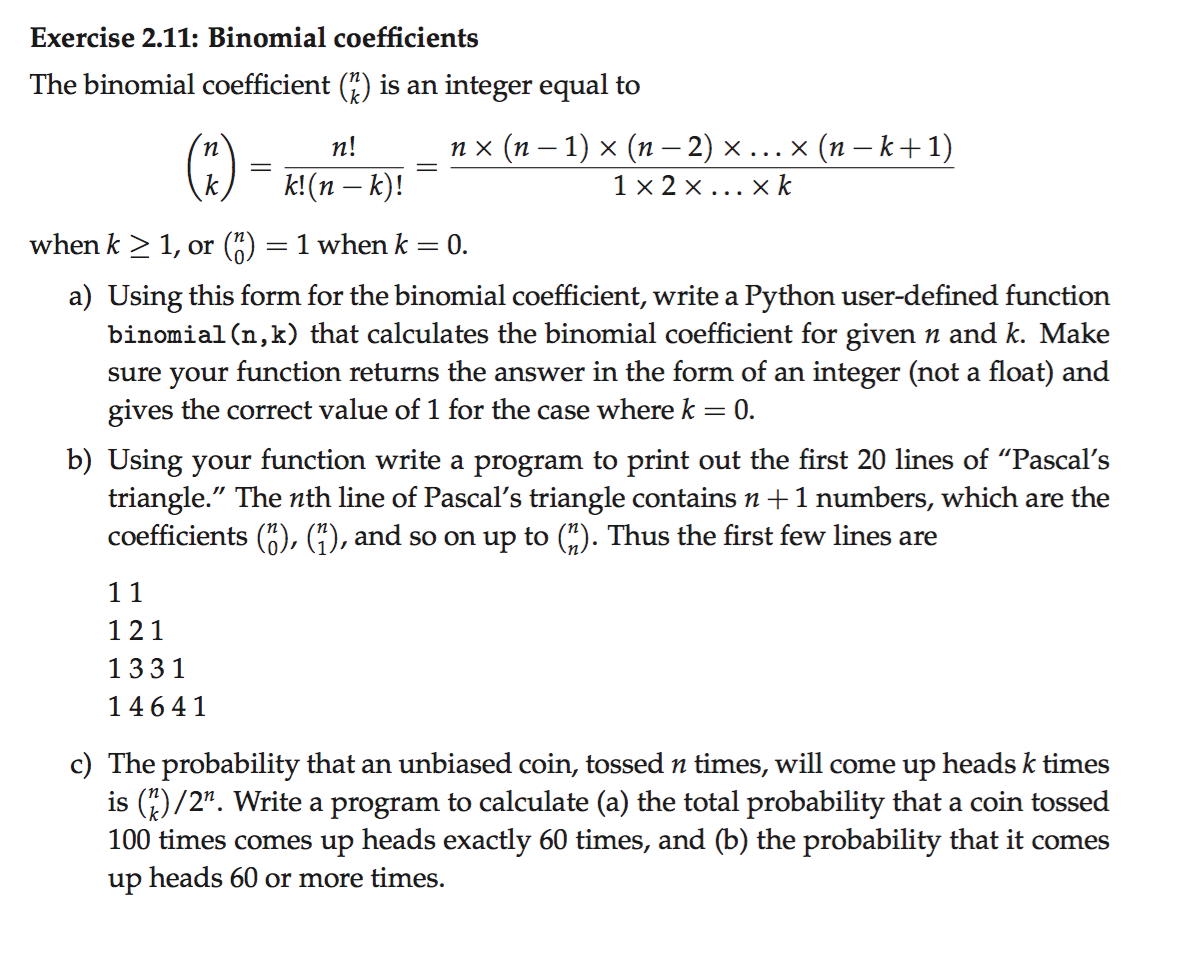
\includegraphics[width=1.0\textwidth]{Exercise2_11.png}%
 %\caption{\label{}}
%\end{figure*}

%%%%%%%%%%%%%%%%%%%%%%%%%%%%%%%%%%%%%%%%%%%%%%%%%%%%%%%%%%%%%%%%%%%%%%%%%%%%%


%%%%%%%%%%%%%%%%%%%%%%%%%%%%%%%%%%%%%%%%%%%%%%%%%%%%%%%%%%%%%%%%%%%%%%%%%%%%%
% Place all of the references you used to write this paper in a file
% with the same name as following the \bibliography command
%%%%%%%%%%%%%%%%%%%%%%%%%%%%%%%%%%%%%%%%%%%%%%%%%%%%%%%%%%%%%%%%%%%%%%%%%%%%%

\bibliography{sample-paper}

\bibliographystyle{prsty}
\begin{thebibliography}{}
\bibitem{newman} Newman, M., Computational Physics - Revised and Expanded, [2013] 
\bibitem{whypython} Why Python: http://lorenabarba.com/blog/why-i-push-for-python, [2014]
\bibitem{jupyter} Jupyter Notebooks: http://jupyter.org/, [2017]
\bibitem{github} GitHub: https://github.com, [2017]
%\bibitem{melissinos2003}Melissinos, A.C., Napolitano, J.,  Experiments in Modern
%  Physics - 2nd Edition, Academic Press,  [2003]
%\bibitem{bevington2003}Bevington and Robinson, Data Reduction and
%  Error Analysis for the Physical Sciences - 3rd Edition, McGraw-Hill,
%  [2003]
%\bibitem{pritchard1990}Professor D. Pritchard, Personal Communication
\end{thebibliography}


\end{document}
%
% ****** End of file apssamp.tex ******